\chapter{Goals and Scope}

The platform will integrate sophisticate hardware and software elements that allow us to deploy a
remote controlled robot so that it can be used by students in a game platform using the provided
user interface.

The development of the project will require knowledge about the hardware (for the maintenance and
modifications of the robot), knowledge about communication protocols (\acrlong{http} or
\acrshort{http}, \acrshort{tcp}/\acrshort{ip} and Bluetooth) for command and image transmission,
knowledge about web engineering (for the development of the client and the interaction with the
WebLab-Deusto platform) and user interface design knowledge for creating a user-friendly interface
taking into account the requirements asked by the ``\acrlong{fecyt}'' (\acrshort{fecyt}) ``Ciencia
remota'' initiative.

\section{Project Definition}

The secondary objectives of the project will be the following:
\begin{itemize}
\item \textbf{Requirement analysis, state of the art study. Requirements specification}:

A complete state of the art study will be performed to know th current market situation regarding to
remote robotic laboratories and the \acrshort{stem} promotion in young people. Moreover, a
requirement analysis will be performed which will give us the final requirement specification.

\item \textbf{\acrshort{stem} element revision for young students}:

We will analyze which are the most influential elements in the education of students in the
\acrshort{stem} area so that they can be maximized when developing the platform. They will be proved
with young students aged between 10 and 18 years old.

\item \textbf{Current hardware platform analysis and modification}:

We will study the possibilities of the current hardware in WebLab-Deusto (the robot Romie) and the
needed changes will be developed to adapt it to the needs of the project.

\item \textbf{\acrshort{api} for remote control}):

A complete control \acrshort{api} will be developed, able of communicating with the robot with a
a simple interface for the client software taking into account the restrictions of the WebLab-Deusto
environment.

\item \textbf{Trivia game platform development - registration, game design, score and robot
control}:

A game platform will be created based on a simple trivia game, where the user will have to answer
the proposed questions to obtain a high score. A contest will take place where these users will get
a prize. Game rules must be carefully analyzed so that the game will not be too easy nor too
difficult.

\item \textbf{Integration of a psychological experiment for fighting against pseudoscience. Work
with a psychologist group}:

The psychology laboratory of the University of Deusto, Labpsico will provide an experiment about the
fight against pseudoscience that will be added to the game in one of its game modes. The relevant
data for the psychological research will be sent to Labpsico, while the user will receive a bonus in
the game depending on his or her performance in the psychological activity.

\item \textbf{Visual programming environment for the robot}:

A visual programming environment for the robot will be created based on one of the most known
platforms: Blockly or Scratch, still to be decided, depending on the previous research. This
environment will be used to teach the basics of programming to young students.

\item \textbf{Integration in WebLab-Deusto}:

We will use the WebLab-Deusto platform provided by the University of Deusto so that we can deploy
the experiment in a production environment along with the rest of the experiments. This provides the
experiment with a simple interface for the communication with the experiment server and with the
robot. It will also be in charge of managing user queues and user authentication.

\item \textbf{Platform dissemination: Deployment in the ``Ciencia Remota'' project of
\acrshort{fecyt} and testing by students}:

The game will be deployed in th ``Ciencia Remota'' projct of \acrshort{fecyt} where many
institutions work to bring remote experimentation to more places. For that, and as a demonstration
of the potential of the project, some public test will be performed where students from various
schools will take part.

\item \textbf{Usage statistics report}:

A complete report will be generated to learn from the use statistics. This will provide us with
information on how to improve the game.

\end{itemize}

\section{Description of the Embodiment}

\subsection{Development Methodology}

\begin{figure}
	\centering
	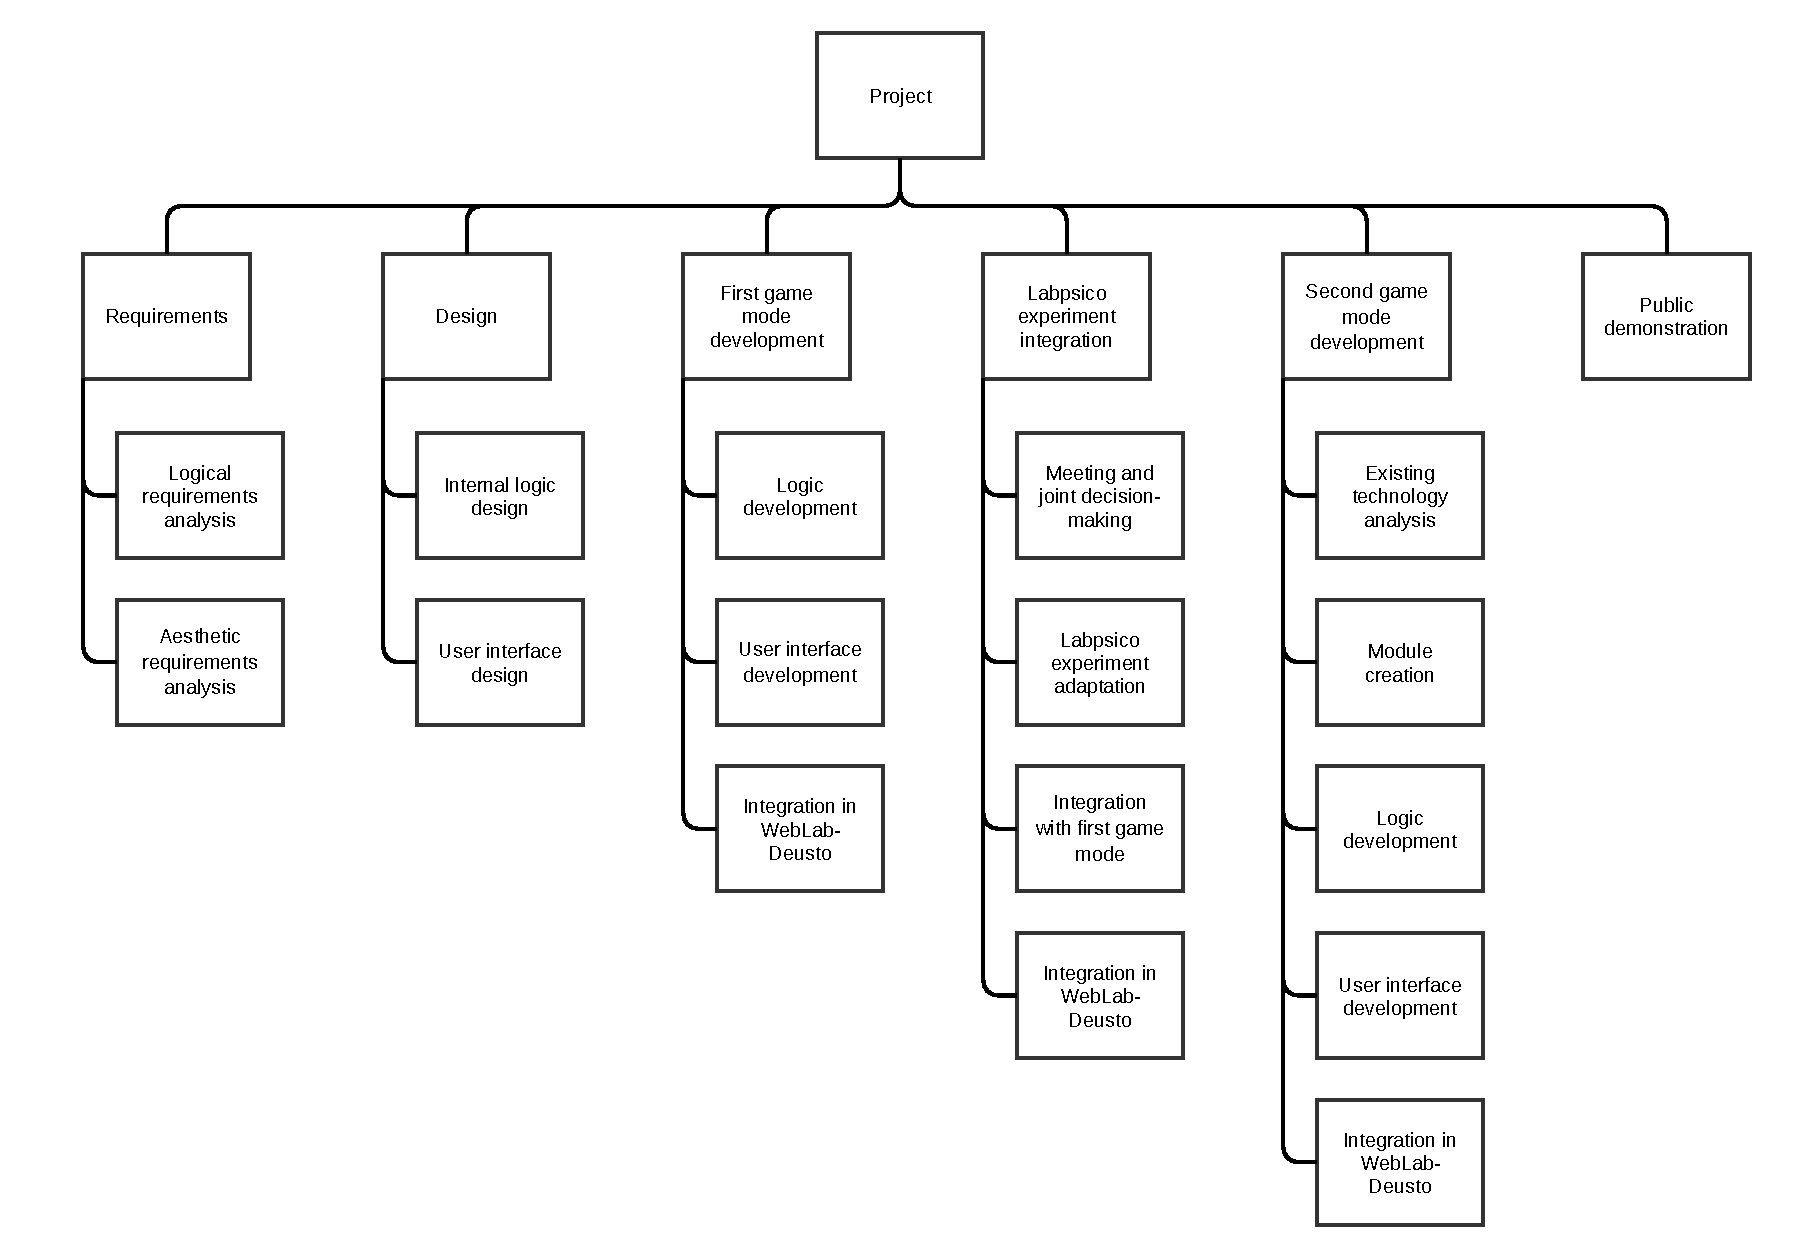
\includegraphics[height=0.9\textwidth, angle=90]{fig/wbs}
	\caption{Project's \acrlong{wbs}.}\label{fig:wbs}
\end{figure}

In the project's \acrlong{wbs} or \acrshort{wbs} (figure~\ref{fig:wbs}) we can see how the project
will be developed, and how the task will be divided. As we can see in the \acrshort{wbs}, the phases
of the project will be the following:

\begin{itemize}
\item \textbf{Requirements}: Project's requirements analysis, in which functional and aesthetic
requirements will be determined.

\item \textbf{Design}: Comprehensive design of the project, both functional and aesthetic, to define
the final product.

\item \textbf{First game mode development}: The first intermediate product will be developed, and it
will be integrated in the WebLab-Deusto platform. This game will be a trivia type game.

\item \textbf{Labpsico experiment integration}: An experiment provided by the University of Deusto's
psychology laboratory, Labpsico, will be integrated with the first game mode.

\item \textbf{Second game mode development}: The second game mode will be developed, based on visual
programming, to teach computing logic.

\item \textbf{Public demonstration}: A public demonstration will be performed to test the viability
and reliability of the project with students.
\end{itemize}

\subsection{Intermediate Products}

These will be the intermediate products that the project will produce:

\begin{itemize}
\item \textbf{First game mode}: This game mode will be a trivia game, where the user will move the
robot in a labyrinth and will have to replay questions in specific location.

\item \textbf{First game mode with Labpsico experiment}: The same game mode as the one before will
be modified to accommodate the experiment provided by Labpsico, based on a psicology experiment
to fight against pseudoscience.

\item \textbf{Second game mode}: A second game mode will be created where users will be able to
program actions to the robot and make it move around the labyrinth.
\end{itemize}

\subsection{Main Tasks}

\subsubsection{Requirements}

\begin{itemize}
\item \textbf{T1 - Logical requirements analysis}: A detailed analysis will be performed to
understand all the functional requirements of the platform. That way we will be able to track them
and check its fulfillment.

\item \textbf{T2 - Aesthetic requirements analysis}: A detailed analysis will be performed to
understand all the aesthetic requirements of the platform. That way we will be able to track them
and check its fulfillment.
\end{itemize}

\subsubsection{Design}

\begin{itemize}
\item \textbf{T3 - Internal logic design}: The internal logic of the robot and the control platform
have to be designed in thinking on accessibility, stability and simplicity.

\item \textbf{T4 - User interface design}: The \acrlong{ui} of the platform has to be designed
thinking on the final user, so that the robot is easy to control.
\end{itemize}

\subsubsection{First game mode development}

\begin{itemize}
\item \textbf{T5 - Logic development}: The internal logic of the trivia game will be developed
thinking always on the modularity and extensibility.

\item \textbf{T6 - User interface development}: A \acrlong{ui} will be developed taking into account
usability standards to use the robot and answer questions.

\item \textbf{T7 - Integration in WebLab-Deusto}: The game platform will be integrated in
WebLab-Deusto using its queue and priority management systems.
\end{itemize}

\subsubsection{Labpsico experiment integration}

\begin{itemize}
\item \textbf{T8 - Meeting and joint decision making}: We will have a meeting with the psychology
laboratory of the University of Deusto, Labpsico, where we will decide how to integrate their
experiment with the first game mode.

\item \textbf{T9 - Labpsico experiment adaptation}: The experiment provided by Labpsico will be
adapted to make sense in the experiment with the robot.

\item \textbf{T10 - Integration with first game mode}: The experiment will be integrated with the
existing platform with the robot using the interface created for the first game mode.

\item \textbf{T11 - Integration in WebLab-Deusto}: The new game will be integrated in WebLab-Deusto
using its queue and priority management systems.
\end{itemize}

\subsubsection{Second game mode development}

\begin{itemize}
\item \textbf{T12 - Existing technology analysis}: A detailed analysis will be performed to decide
which visual programming tool will be the one used for this game mode.

\item \textbf{T13 - Module creation}: The modules needed for controlling the robot will be created.

\item \textbf{T14 - Logic development}: The game logic will be developed so that the program created
by the user can control the robot.

\item \textbf{T15 - User interface development}: A simple \acrlong{ui} will be developed to be able
to use all the functions of the visual programming mode.

\item \textbf{T16 - Integration in WebLab-Deusto}: The visual programming environment will be
integrated in WebLab-Deusto using its queue and priority management systems.
\end{itemize}

\subsubsection{Public demonstration}

\begin{itemize}
\item \textbf{T17 - Public demonstration}: At least one public demonstration of the robot will be
performed during its development where students will try it and play with it.
\end{itemize}

\section{Organization}

\subsection{Organizational Structure}

The working team, as it can be seen in the figure~\ref{fig:org}, it will be organized in a direction
committee, that will be in charge of the good progress of the project, as well as of indicating
the possible needed changes, and in a development team, that will be in charge of developing the
project. Moreover, in the integration of the Labpsico experiment, the Labpsico team will be part of
the project organization team to validate the progress.

\begin{figure}[ht]
	\centering
	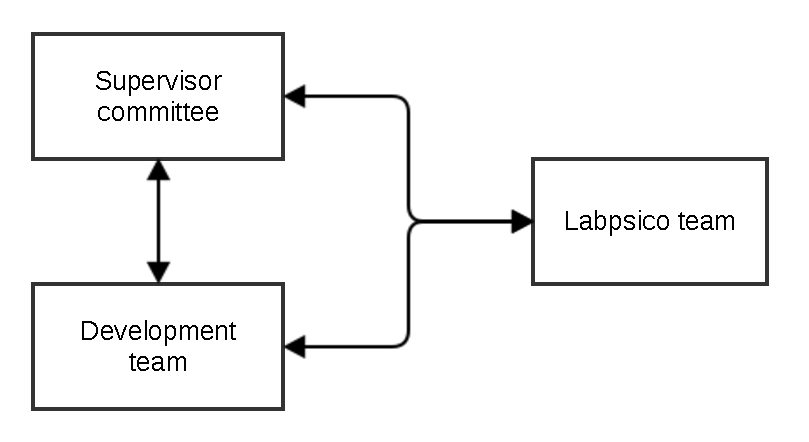
\includegraphics[width=0.7\textwidth]{fig/organization}
	\caption{Project's organization schema.}\label{fig:org}
\end{figure}

\subsection{Human Resources Plan}

The workday will be part time, 4 hours and we will only have one resource, that will be divided into
the following profiles:

\begin{itemize}
\item One \textbf{project manager}: he will be the person in charge of organizing the project.

\item One \textbf{programmer}: he will be the person in charge of developing the logic of the
software.

\item One \textbf{designer}: he will be the person in charge of designing and creating a
\acrlong{ui} intuitive and simple.

\item One \textbf{WebLab-Deusto expert}: he will be in charge of the integration of the experiment
in WebLab-Deusto.
\end{itemize}

Regular meetings will be done, at least twice a month to track the project progress. To validate the
various modules of the application, we will check if the established requirements are met, and
volunteers of the team will perform the needed testing. The organization of the working team will
not be hierarchical but rather horizontal, to allow a much more agile development.
